\documentclass[12pt,fleqn]{article}\usepackage{../../common}
\begin{document}
Konusma Tanima (Speech Recognition)

CTC

\inputminted[fontsize=\footnotesize]{python}{train_ctc.py}

Frekans Uzerinden Ozellik Cikartimi, RNN, LSTM, GRU

\begin{minted}[fontsize=\footnotesize]{python}
import util
import scipy.io.wavfile, zipfile
import io, time, os, random, re

f = util.train_dir + '/down/004ae714_nohash_0.wav'
wav = io.BytesIO(open(f).read())
v = scipy.io.wavfile.read(wav)
print v[1]
#scipy.io.wavfile.write('/tmp/tmp1.wav', util.fs, vnew)    
plt.plot(v[1])
plt.savefig('speech_01.png')
\end{minted}

\begin{verbatim}
[-130 -135 -131 ..., -154 -190 -224]
\end{verbatim}

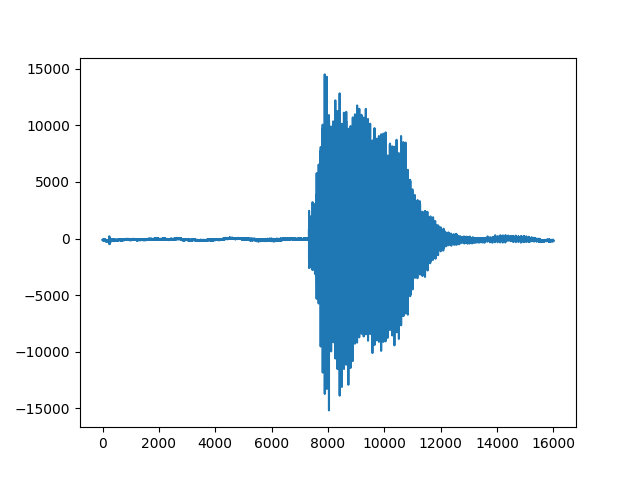
\includegraphics[width=20em]{speech_01.png}

\begin{minted}[fontsize=\footnotesize]{python}
plt.specgram(v[1], Fs=util.fs, NFFT=1024)
plt.savefig('speech_02.png')
\end{minted}

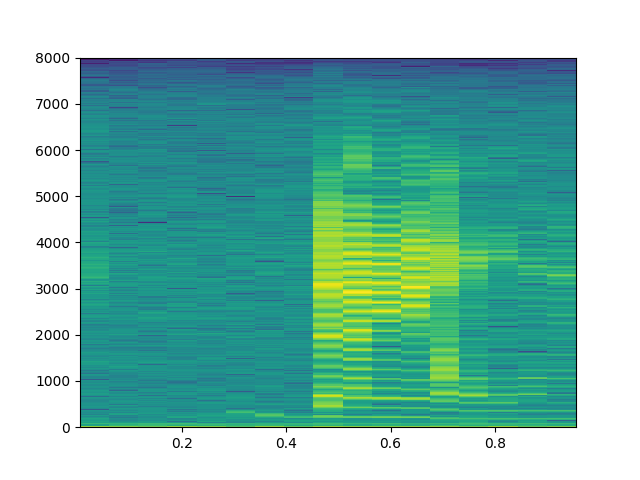
\includegraphics[width=20em]{speech_02.png}

\begin{minted}[fontsize=\footnotesize]{python}
f1 = util.train_dir + '/down/0f3f64d5_nohash_2.wav'
wav1 = io.BytesIO(open(f1).read())
v1 = scipy.io.wavfile.read(wav1)
plt.specgram(v1[1], Fs=util.fs, NFFT=1024)
plt.savefig('speech_03.png')

f2 = util.train_dir + '/no/01bb6a2a_nohash_0.wav'
wav2 = io.BytesIO(open(f2).read())
v2 = scipy.io.wavfile.read(wav2)
plt.specgram(v2[1], Fs=util.fs, NFFT=1024)
plt.savefig('speech_04.png')
\end{minted}

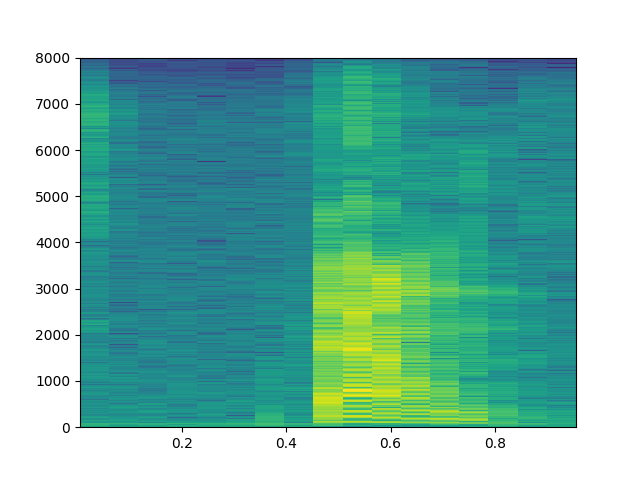
\includegraphics[width=20em]{speech_03.png}
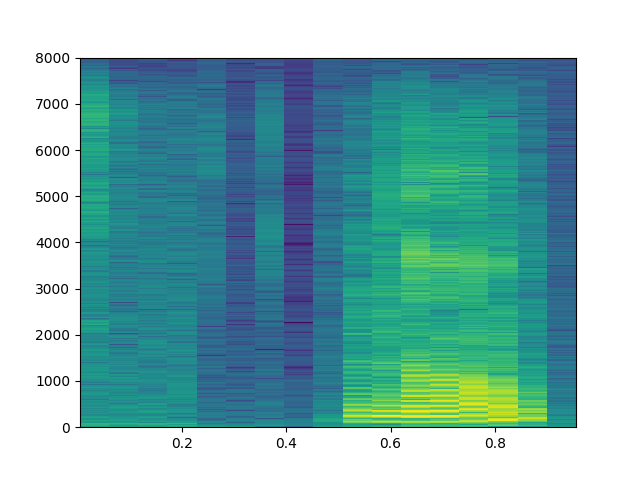
\includegraphics[width=20em]{speech_04.png}


\inputminted[fontsize=\footnotesize]{python}{train_rnn.py}


[devam edecek]



Kaynaklar

[1] Bayramli, {\em VCTK Ses Tanima Verisi, Konusmaci 225}, \url{https://www.dropbox.com/s/xecprghgwbbuk3m/vctk-pc225.tar.gz?dl=1}

[2] Remy, {\em Application of Connectionist Temporal Classification (CTC) for Speech Recognition},\url{https://github.com/philipperemy/tensorflow-ctc-speech-recognition}

[3] Graves, {\em Supervised Sequence Labelling with Recurrent Neural Networks}, \url{https://www.cs.toronto.edu/~graves/preprint.pdf}

[4] Graves, {\em How to build a recognition system (Part 2): CTC Loss}, \url{https://docs.google.com/presentation/d/12gYcPft9_4cxk2AD6Z6ZlJNa3wvZCW1ms31nhq51vMk}

[5] Graves, {\em How to build a recognition system (Part 1): CTC Loss}, \url{https://docs.google.com/presentation/d/1AyLOecmW1k9cIbfexOT3dwoUU-Uu5UqlJZ0w3cxilkI}

[6] Bayramli, {\em Small Voice Files}, \url{https://www.dropbox.com/s/8754ytatft2ttge/voice_cmd_small.zip?dl=1}

\end{document}
